% A LaTeX paper with an agent beside you: live preview, no compile queue.
%
% Start here:
%   1. The PDF compiles beside your source as you open this file.
%   2. One \ref below is broken (it renders "??"). Press Cmd+J and ask
%      the Agent to fix it. The fix lands as a tracked change you review.
%   3. Paste in your own draft, or drop your project into this folder.
\documentclass{article}
\usepackage{amsmath}
\usepackage{graphicx}
\usepackage{tikz}
\usetikzlibrary{arrows.meta,positioning,shapes.geometric}

\title{An Inspectable Design-to-Screen Agent for De Novo Protein Campaign Downselection}
\author{re:AGENT Hackathon Team}
\date{}

\begin{document}
\maketitle

\begin{abstract}
Modern generative protein-design systems can propose thousands of structurally plausible candidates, but experimental expression, binding, developability, and HLA testing remain limiting steps. We present an inspectable scientific-agent workflow intended to reduce this design-to-experiment gap by combining literature-grounded design specifications, versioned de novo generation, structural triage, and human HLA-A*02:01 binding and presentation evidence. Overlapping 9-mers are represented by a frozen ESM-2 650M encoder, and a compact-student workflow is configured to imitate separate NetMHCpan 4.1 eluted-ligand (EL) and binding-affinity (BA) channels on Protein Design Archive sequences. Existing cleavage and TAP heads remain separate, and the processing composite is the geometric mean of N-terminal cleavage, C-terminal cleavage, and BA binding propensity; EL presentation and TAP are reported separately. The completed full-PDA corpus contains 160,012 unique peptides with frozen 1,280-dimensional embeddings. Across five component-grouped held-out folds, EL and BA predictions reached mean Spearman correlations of 0.9431 and 0.9478 against teacher rank, respectively. On 159,038 unique PDA peptides scored against the same NetMHCpan EL teacher, the legacy Chao1 MHCflurry head achieved strong-binder average precision 0.060, while the out-of-fold student achieved 0.820. We also demonstrate provenance-preserving orchestration and sequence-to-structure visualization on one 99-residue de novo protein. These metrics measure teacher imitation. Direct validation requires measured human HLA-A*02:01 affinity for BA and human HLA-A*02:01 immunopeptidomics for EL and the processing stack. The system does not predict TCR recognition or a whole immune response.
\end{abstract}

\section{Introduction}
Computational protein design has entered a high-throughput regime in which massively parallel generation and design-build-test-learn cycles can produce and evaluate large candidate libraries \cite{silva2018miniproteins}. RFdiffusion enables target- and hotspot-conditioned backbone generation, while ProteinMPNN efficiently samples sequences compatible with designed backbones \cite{watson2023rfdiffusion,dauparas2022proteinmpnn}. The Protein Design Archive provides a curated corpus of de novo designed protein sequences and structures \cite{chronowska2025pda}. This growing design capacity creates a practical asymmetry: candidate generation is increasingly inexpensive, while experimental characterization remains slow and resource intensive.

HLA class I presentation requires several distinct events: an intracellular protein is proteolytically processed, a peptide is transported, the peptide binds an HLA molecule, and the resulting complex reaches the cell surface. BA describes only peptide--HLA binding. EL is presentation-oriented because its training evidence includes naturally eluted ligands and therefore information from upstream processing \cite{reynisson2020netmhc}. Neither output predicts TCR recognition or whether a peptide is perceived as dangerous. Keeping these endpoints separate is essential when using predictions to prioritize experimental work.

\subsection{Machine-learning precedent}
The computational strategy follows two established machine-learning patterns. Foundation models are pretrained on broad data and subsequently adapted to many downstream tasks \cite{bommasani2021foundation}. Knowledge distillation trains a student against outputs from a more cumbersome teacher so that task-specific behavior can be reproduced in a more deployable model \cite{hinton2015distilling}. DistilBERT illustrates full model compression by reducing the teacher encoder itself \cite{sanh2019distilbert}. Our implementation is different: NetMHCpan supplies pseudo-labels, frozen ESM-2 supplies peptide representations, and a compact multilayer head learns the task mapping. This is feature-based task distillation, not end-to-end compression of ESM-2.

The same transfer pattern appears across scientific foundation models. Protein language models learn reusable sequence representations; the Nucleotide Transformer adapts DNA representations to genomic prediction tasks; and scGPT adapts a generative model trained across millions of cells to several single-cell tasks \cite{lin2023esm2,dallatorre2024nucleotide,cui2023scgpt}. These examples support the general technique of pairing broad self-supervised representations with small supervised adapters. They do not establish that the transferred representation or teacher remains calibrated on designed proteins, so distribution-shift and external-validation requirements remain part of our method.

Our premise is that an agent can narrow a large de novo campaign to a smaller, traceable set of candidates before expensive experiments. Paperclip converts literature into cited design and validation constraints; Proto executes RFdiffusion3, ProteinMPNN, and structure-prediction tools; and a LangGraph workflow records artifacts, enforces approval and reviewer gates, and renders peptide-level evidence in a scientific workbench. The output is a prioritization dossier that helps scientists decide what to express and which peptide--HLA measurements to run next.

\section{Methods}
\subsection{Generation constraints}
RFdiffusion established that target structures and interface hotspots can condition de novo binder generation \cite{watson2023rfdiffusion}. We applied the newer all-atom RFdiffusion3 model through Proto on Modal \cite{butcher2025rfdiffusion3}, then used ProteinMPNN to sample sequences compatible with each generated backbone \cite{dauparas2022proteinmpnn}. AlphaFold provides an independent refolding and interface-confidence check. Each target used a pinned PDB structure, literature- or complex-derived hotspots, two binder-length ranges (55--85 and 85--120 residues), and fixed low-temperature inference settings. The published in silico gates, monomer pLDDT above 80, interaction PAE below 10, and designed-to-refolded binder RMSD below 1 \AA, are treated as triage thresholds rather than proof of binding.

\subsection{Service architecture}
The services have non-overlapping roles. Paperclip turns literature into cited design and validation constraints. Proto executes versioned biological tools and records their inputs, seeds, configurations, runtimes, and artifacts. IEDB provides live NetMHCIIpan EL and BA predictions. The local agent joins these outputs through typed adapters, records provenance, and renders sequence and structure-linked evidence. BenchFlow can package the validation lanes as separate frozen tasks with deterministic verifiers; it evaluates reproducibility and task completion, but does not create biological ground truth.

\begin{figure}[t]
\centering
\resizebox{\textwidth}{!}{%
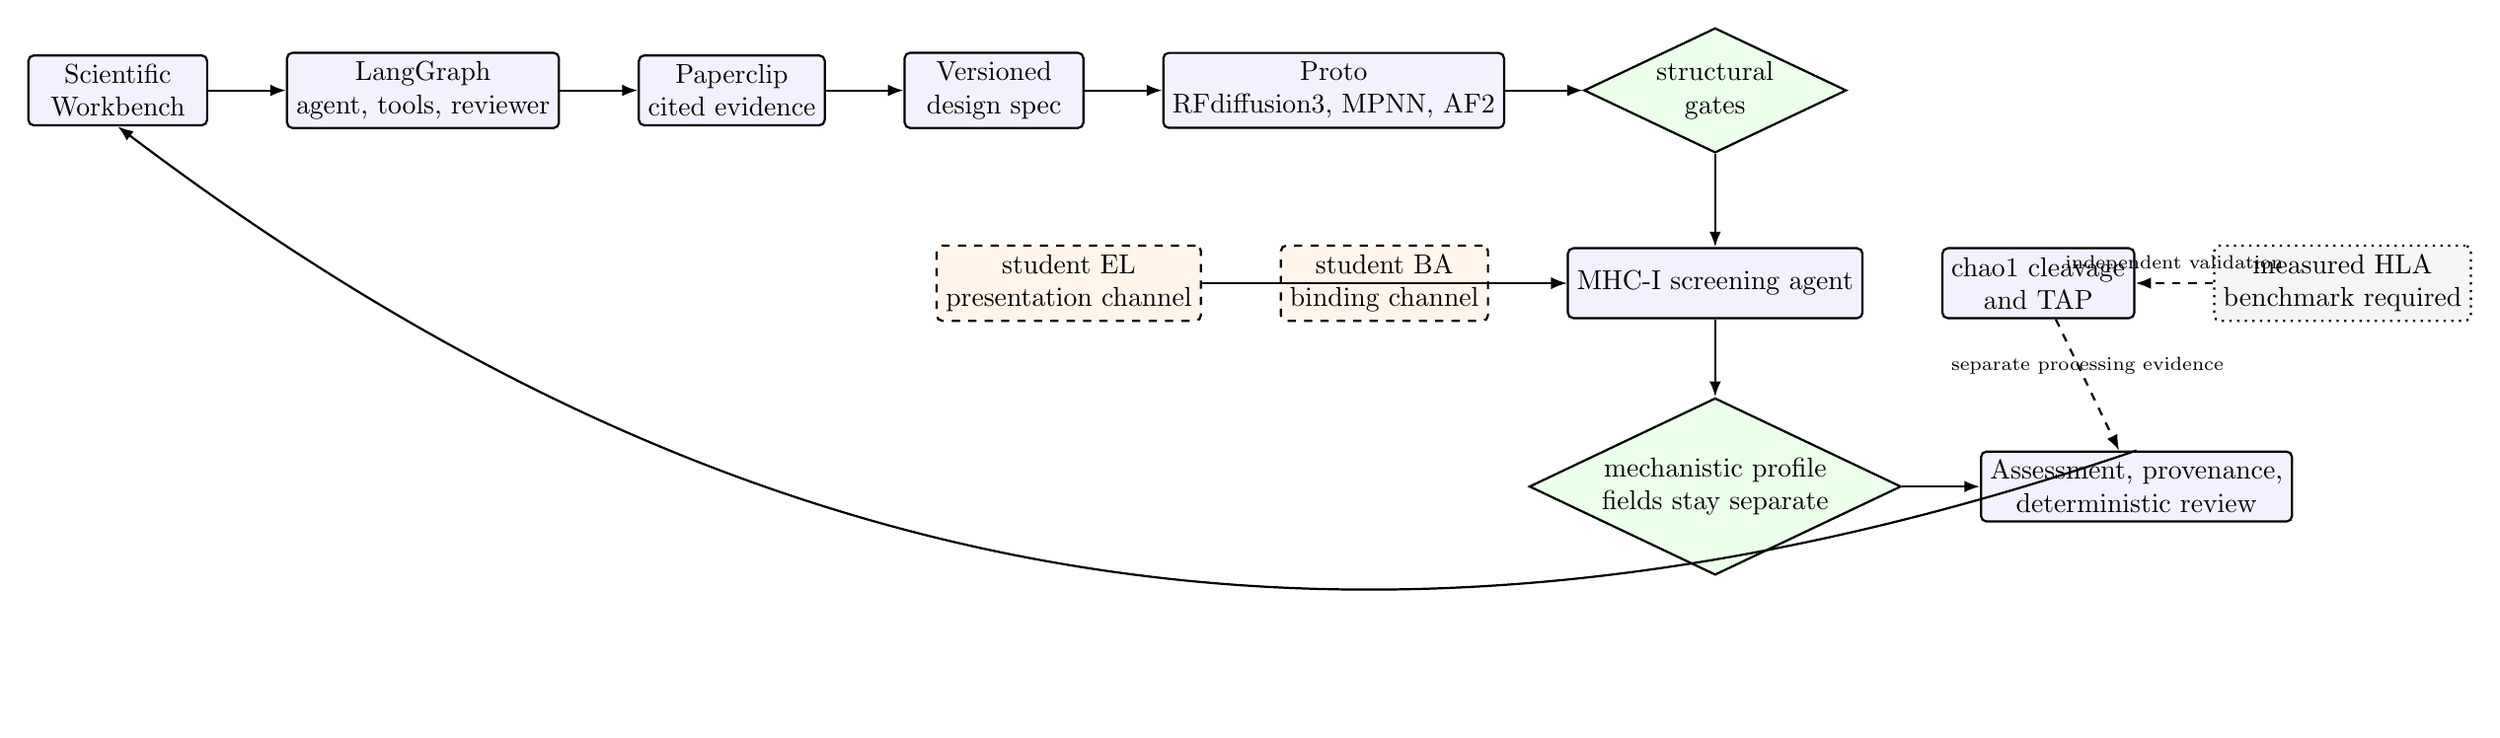
\begin{tikzpicture}[
  node distance=7mm and 10mm,
  implemented/.style={draw, thick, rounded corners=2pt, align=center, minimum height=9mm, minimum width=23mm, fill=blue!5},
  replay/.style={implemented, dashed, fill=orange!8},
  offline/.style={implemented, dotted, fill=gray!8},
  gate/.style={draw, thick, diamond, aspect=2.1, align=center, inner sep=1.5pt, fill=green!8},
  arr/.style={-{Latex[length=2mm]}, thick},
  sep/.style={-{Latex[length=2mm]}, thick, dashed}
]
\node[implemented] (ui) {Scientific\\Workbench};
\node[implemented, right=of ui] (graph) {LangGraph\\agent, tools, reviewer};
\node[implemented, right=of graph] (paper) {Paperclip\\cited evidence};
\node[implemented, right=of paper] (spec) {Versioned\\design spec};
\node[implemented, right=of spec] (proto) {Proto\\RFdiffusion3, MPNN, AF2};
\node[gate, right=of proto] (struct) {structural\\gates};

\node[implemented, below=12mm of struct] (screen) {MHC-I screening agent};
\node[replay, left=of screen] (ba) {student BA\\binding channel};
\node[replay, left=of ba] (el) {student EL\\presentation channel};
\node[implemented, right=of screen] (chao) {chao1 cleavage\\and TAP};
\node[offline, right=of chao] (measured) {measured HLA\\benchmark required};
\node[gate, below=10mm of screen] (fusion) {mechanistic profile\\fields stay separate};
\node[implemented, right=of fusion] (dossier) {Assessment, provenance,\\deterministic review};

\draw[arr] (ui) -- (graph);
\draw[arr] (graph) -- (paper);
\draw[arr] (paper) -- (spec);
\draw[arr] (spec) -- (proto);
\draw[arr] (proto) -- (struct);
\draw[arr] (struct) -- (screen);
\draw[arr] (ba) -- (screen);
\draw[arr] (el) -- (screen);
\draw[arr] (screen) -- (fusion);
\draw[arr] (fusion) -- (dossier);
\draw[sep] (chao) -- node[above, font=\scriptsize] {separate processing evidence} (dossier);
\draw[sep] (measured) -- node[above, font=\scriptsize] {independent validation} (chao);
\draw[arr, bend left=28] (dossier.north) to (ui.south);
\end{tikzpicture}%
}
\caption{Inspectable design-to-screen architecture. Solid boxes are implemented in the LangGraph workbench path, dashed boxes use cached or frozen artifacts, and dotted boxes denote missing direct experimental validation. Literature constrains generation rather than directly generating a valid protein. Structural gates precede separate HLA-A*02:01 BA, EL, cleavage, and TAP evidence. Independent affinity and ligand-presentation measurements remain required.}
\label{fig:agent-architecture}
\end{figure}

\subsection{Frozen protein-language representations and processing heads}
The MHC-I lane uses final-layer residue representations from \texttt{esm2\_t33\_650M\_UR50D}, a 33-layer protein language model with 1,280-dimensional embeddings. Prior work supports transfer of ESM representations to peptide-MHC prediction, although published systems commonly fine-tune the encoder and include an MHC pseudo-sequence \cite{hashemi2023plm}. Our implementation instead freezes ESM-2 and trains compact task heads, reducing the number of trainable parameters, avoiding repeated teacher calls, and making the learned adapter easy to version. Inference still requires the 650M-parameter ESM-2 encoder, so the current system is not a fully compressed small model. A genuinely compact deployment would also distill or replace the encoder. Freezing ESM-2 creates an explicit domain-shift caveat because it was pretrained primarily on natural full-length proteins rather than designed proteins and isolated 9-mers.

The legacy \texttt{chao1} checkpoint supplies independently trained N- and C-terminal cleavage heads and a relative TAP transport head. It was associated with a 5,000,613-row HLA-A*02:01 corpus containing human, bacterial, viral, and de novo peptides, but most cleavage and MHC labels were teacher-derived and only 613 TAP measurements were experimental. The old MHCflurry-derived MHC head is therefore being replaced, while cleavage and TAP remain separately reported processing evidence. The checkpoint is an MHC-I surrogate, not an MHC-II, CD4-response, or human-immunogenicity model.

\subsection{Full-PDA NetMHCpan distillation}
The replacement student is trained on the full Protein Design Archive distribution rather than treating PDA as an external benchmark. Every overlapping 9-mer from every PDA parent is first labeled with NetMHCpan 4.1 EL and BA outputs. Exact peptide duplicates are then collapsed while retaining occurrence and parent counts. Parents sharing any exact 9-mer are connected into components, and each connected component is assigned wholly to one of five folds. Greedy fold balancing uses unique-peptide count, preventing direct peptide leakage while retaining all available designed-protein parents.

Each 9-mer is represented by the mean of its nine ESM-2 residue vectors, excluding special tokens. A two-output head applies layer normalization, a 256-unit hidden layer with GELU and dropout, and sigmoid EL and BA outputs. Teacher percentile rank $r$ is transformed to a higher-is-riskier propensity
\begin{equation}
  p(r)=1-\frac{\log(1+r)}{\log(101)}, \qquad 0\leq r\leq100.
\end{equation}
Five heads are trained. For each head, one component-grouped fold is untouched test data, the next fold is validation data, and the remaining three folds are training data. Deployment averages the five heads, while reported cross-validation metrics use only out-of-fold predictions. These metrics quantify NetMHCpan imitation, not biological accuracy.

\begin{figure}[t]
\centering
\resizebox{\textwidth}{!}{%
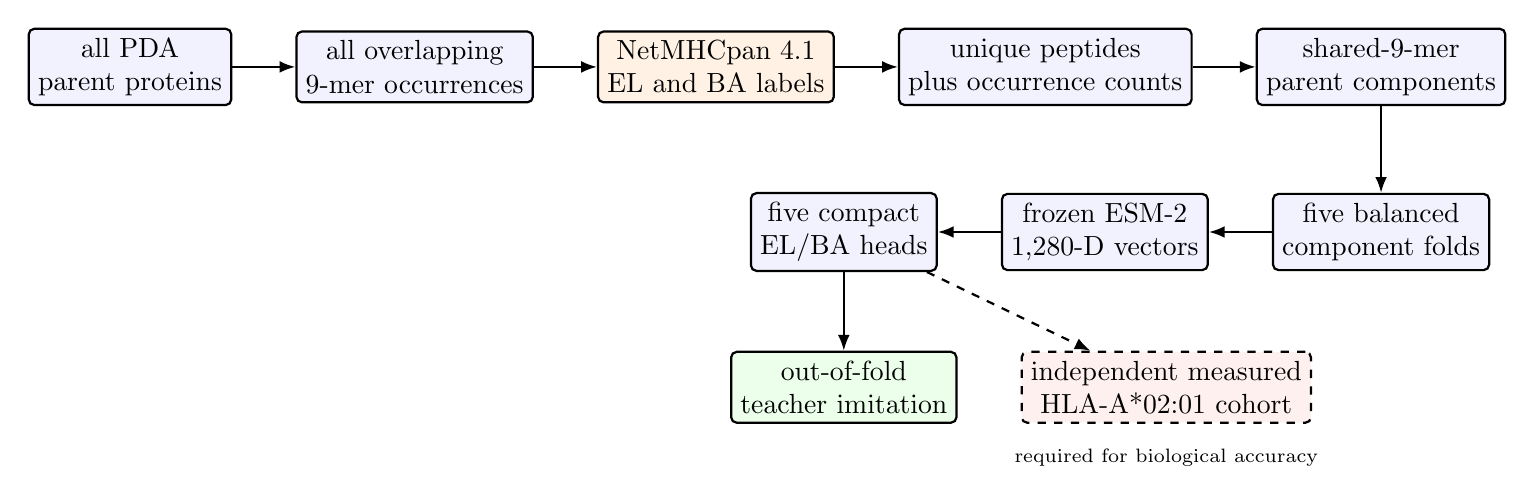
\begin{tikzpicture}[
  node distance=7mm and 8mm,
  stage/.style={draw, thick, rounded corners=2pt, align=center, minimum height=9mm, minimum width=23mm, fill=blue!5},
  teacher/.style={stage, fill=orange!10},
  eval/.style={stage, fill=green!8},
  caution/.style={stage, dashed, fill=red!6},
  arr/.style={-{Latex[length=2mm]}, thick}
]
\node[stage] (parents) {all PDA\\parent proteins};
\node[stage, right=of parents] (tile) {all overlapping\\9-mer occurrences};
\node[teacher, right=of tile] (api) {NetMHCpan 4.1\\EL and BA labels};
\node[stage, right=of api] (dedup) {unique peptides\\plus occurrence counts};
\node[stage, right=of dedup] (graph) {shared-9-mer\\parent components};
\node[stage, below=11mm of graph] (folds) {five balanced\\component folds};
\node[stage, left=of folds] (embed) {frozen ESM-2\\1,280-D vectors};
\node[stage, left=of embed] (heads) {five compact\\EL/BA heads};
\node[eval, below=10mm of heads] (test) {out-of-fold\\teacher imitation};
\node[caution, right=of test] (external) {independent measured\\HLA-A*02:01 cohort};
\draw[arr] (parents) -- (tile);
\draw[arr] (tile) -- (api);
\draw[arr] (api) -- (dedup);
\draw[arr] (dedup) -- (graph);
\draw[arr] (graph) -- (folds);
\draw[arr] (folds) -- (embed);
\draw[arr] (embed) -- (heads);
\draw[arr] (heads) -- (test);
\draw[arr, dashed] (heads) -- (external);
\node[font=\scriptsize, align=center, below=2mm of external] {required for biological accuracy};
\end{tikzpicture}%
}
\caption{Full-PDA NetMHCpan student workflow. Exact shared 9-mers connect parent proteins before five-fold assignment, preventing direct peptide leakage across cross-validation folds. Held-out folds measure teacher imitation. Because the entire PDA corpus supplies training data across the ensemble, a separate non-PDA experimental cohort is required for out-of-distribution and biological-accuracy claims.}
\label{fig:netmhcpan-lineage}
\end{figure}

\subsection{MHC-I risk calculation}
For each 9-mer $i$, the student reports EL presentation propensity $p_{EL,i}$ and BA binding propensity $p_{BA,i}$. Predicted percentile ranks are deterministic inversions of the target transform. EL rank at or below 0.5 is labeled strong, rank above 0.5 and at or below 2.0 is labeled weak, and larger rank is labeled nonbinder. EL and BA are not averaged together because the channels are correlated and EL already includes presentation information. BA enters the current processing heuristic alongside cleavage, while EL and TAP remain separately reported evidence lanes.

The processing score combines the legacy cleavage heads with the replacement BA head:
\begin{equation}
 R_i=\exp\left(\frac{\log \tilde p_{N,i}+\log \tilde p_{C,i}+\log \tilde p_{BA,i}}{3}\right),
 \qquad \tilde p=\max(p,10^{-6}).
\end{equation}
For a protein with $n$ windows, the displayed summary is the mean of the $K=\min(5,n)$ largest $R_i$ values. TAP score, TAP uncertainty, EL propensity, the maximum window score, and residue-level projections are reported separately. This composite is a transparent prioritization heuristic, not a calibrated pathway probability.

\subsection{Mechanistic scope}
The modeled endpoint is restricted to human HLA peptide binding and presentation-related processing, not a whole immune response. NetMHCpan BA estimates the single event of peptide--HLA binding; it does not measure proteolytic generation, surface presentation, T-cell recognition, or whether a peptide is perceived as dangerous. NetMHCpan EL is a distinct, presentation-oriented channel trained with mass-spectrometry eluted-ligand evidence and therefore incorporates information about upstream antigen-processing steps \cite{reynisson2020netmhc}. The inherited cleavage and TAP outputs remain separate mechanistic hypotheses. Downstream T-cell activation, cytokines, antibody responses, and animal outcomes are outside the model target and outside the primary benchmark.

\subsection{Validation architecture}
The orchestration layer accepts immutable model artifacts through versioned, capability-typed adapters. Validation follows the semantics of each output. BA must be compared with independent measured HLA-A*02:01 binding affinity, preferably quantitative IC50 or $K_d$ on canonical 9-mers. EL must be compared with independent human HLA-A*02:01 eluted-ligand or monoallelic immunopeptidomics data using source-protein-aware negatives. The cleavage-plus-BA composite requires a separate ablation against naturally presented ligands because binding affinity alone cannot validate peptide generation. Protein Design Archive sequences supply the component-grouped five-fold distillation corpus \cite{chronowska2025pda}. PDA folds measure teacher imitation, but because all folds contribute to the deployed ensemble, a separate non-PDA experimental cohort is required for biological accuracy.

These endpoints remain a vector rather than an average of incompatible evidence. Exact sequence hashes gate every residue-to-structure visualization. T-cell activation, PBMC cytokines, anti-drug antibodies, and animal outcomes are excluded from primary model evaluation because they add downstream mechanisms that the model does not represent.

\section{Results}
\subsection{Design and orchestration}
The reviewed RFdiffusion3 branch summary reports 100 backbone complexes for each of five targets, for 500 candidate backbones. The underlying backbone PDB files were not preserved in that snapshot, so the count demonstrates reported generation scale but is not yet auditable end to end. In a direct PD-L1 control check, 15 of the first 16 backbones contacted all three configured hotspots within 4.5 \AA, and all 16 contacted all three within 6 \AA. These are geometric backbone results only; sequence design, refolding, interface confidence, binding, and immune screening have not yet been completed on those exact generated backbones.

The workbench connects a LangGraph state machine to typed scientific tools, immutable artifact manifests, approval-gated compute, and deterministic reviewer checks. Each MHC-I output remains labeled by mechanism so missing direct evidence is not silently replaced by a downstream assay.

\subsection{MHC-I corpus and student results}
The completed full-PDA corpus contains 1,602 parent proteins and approximately 290,937 overlapping 9-mer occurrences before exact-peptide deduplication. Deduplication produced 160,012 unique peptides with a frozen ESM-2 embedding matrix of shape $160{,}012\times1{,}280$. The earlier parent-batch smoke cache contained 52,901 EL-labeled windows, but the reported model results use the completed EL and BA corpus.

Across five untouched component-grouped test folds, mean EL Spearman correlation against NetMHCpan rank was 0.9431 with population standard deviation 0.0043; mean BA correlation was 0.9478 with standard deviation 0.0043. At the 2-percent binder threshold, mean area under the precision-recall curve was 0.8914 for EL and 0.8595 for BA. Mean propensity MAE was 0.0557 for EL and 0.0448 for BA. Pooled out-of-fold evaluation covered all 160,012 unique peptides. These results establish high teacher-imitation fidelity under exact-9-mer component grouping. They do not establish experimental presentation accuracy. A completed same-row comparison on 159,038 unique profile peptides found strong-binder average precision of 0.060 for the legacy Chao1 MHCflurry head and 0.820 for the out-of-fold student EL head. This comparison measures agreement with the NetMHCpan teacher, not experimental error.

\begin{table}[t]
\centering
\small
\begin{tabular}{lcc}
\hline
Held-out metric & EL channel & BA channel \\
\hline
Cross-validation folds & 5 & 5 \\
Pooled out-of-fold peptides & 160,012 & 160,012 \\
Binder prevalence & $0.0665 \pm 0.0036$ & $0.0341 \pm 0.0026$ \\
Spearman correlation & $0.9431 \pm 0.0043$ & $0.9478 \pm 0.0043$ \\
Binder AUPRC & $0.8914 \pm 0.0090$ & $0.8595 \pm 0.0028$ \\
No-skill AUPRC & 0.0665 & 0.0341 \\
Propensity MAE & $0.0557 \pm 0.0020$ & $0.0448 \pm 0.0019$ \\
Propensity RMSE & $0.0761 \pm 0.0023$ & $0.0660 \pm 0.0022$ \\
\hline
\end{tabular}
\caption{Cross-validated NetMHCpan teacher-imitation results. Values other than pooled peptide count are mean $\pm$ population standard deviation across five component-grouped held-out folds. Binder AUPRC uses the NetMHCpan rank threshold of 2 percent, and the no-skill reference equals binder prevalence. These are teacher-fidelity metrics, not validation of immunogenicity prediction.}
\label{tab:mhci-student-results}
\end{table}

\subsection{Direct comparison with the legacy Chao1 head}
Table~\ref{tab:mhci-student-results} asks how faithfully the frozen-ESM-2 student reproduces NetMHCpan on held-out PDA peptide components. We also compared the legacy Chao1 MHCflurry-derived presentation head and the student EL head on the same 159,038 unique PDA 9-mers. NetMHCpan EL rank at or below 0.5 percent defined 3,956 strong binders. Because positives were only 2.5 percent of peptides, strong-binder average precision was the primary discrimination metric; AUROC is reported as a secondary measure.

\begin{table}[t]
\centering
\small
\begin{tabular}{lrrr}
\hline
MHC-I score & Spearman & Strong AUROC & Strong AP \\
\hline
Legacy Chao1 MHCflurry head & 0.354 & 0.731 & 0.060 \\
NetMHCpan student EL, out of fold & 0.943 & 0.993 & 0.820 \\
\hline
\end{tabular}
\caption{Direct same-row comparison against NetMHCpan 4.1 EL on 159,038 unique PDA peptides. Strong binders use teacher EL rank at or below 0.5 percent. The student improves average precision by about 14-fold under 2.5-percent prevalence. Chao1 was calibrated to MHCflurry, so this is evidence for replacing the MHC head within this screening stack, not an experimental error rate or an immunogenicity endpoint.}
\label{tab:mhci-technique-comparison}
\end{table}

The same-row result justifies replacing the legacy Chao1 MHC head, while retaining its separately supervised cleavage and TAP heads. It does not show that the student exceeds NetMHCpan, because NetMHCpan is the teacher. Independent measured HLA-A*02:01 binding-affinity and eluted-ligand cohorts remain necessary for mechanistic validation.

\subsection{De novo protein demonstration}
We used \texttt{pda:9s14:0}, a 99-residue PDA design in the ``novel'' structural bin with nearest-natural Foldseek TM-score 0.4728, as a traceable visualization example. The legacy \texttt{chao1} adapter scored all 91 overlapping 9-mers. Its top-five mean processing composite was 0.6975, and its maximum was 0.7053 at peptide \texttt{WVLATEIYR}. The parent sequence and all 91 9-mers were absent from the supplied legacy 5,000,613-row teammate parquet.

\begin{figure}[t]
\centering
\includegraphics[width=\textwidth]{figures/workbench.png}
\caption{Scientific Workbench view of the 9S14 de novo protein demonstration. Residue-level processing tracks are linked to the three-dimensional structure and shown beside separate BA, EL, cleavage, TAP, provenance, and reviewer evidence. The reviewer pass verifies artifact completeness and claim boundaries, not biological accuracy. The displayed processing score is a legacy-model smoke inference.}
\label{fig:workbench}
\end{figure}

This demonstration establishes that a complete de novo sequence can be tiled, embedded, scored, mapped back to structure, and reviewed with provenance. It does not establish generalization of the new PDA-trained student. Once the full PDA corpus is used for training, PDA examples including 9S14 cannot serve as external OOD validation unless their complete connected component is excluded from every deployed head.

\subsection{Mechanistic benchmark required}
The current external NY-ESO-1 cohort is useful for out-of-corpus teacher fidelity, but its T-cell activation labels are downstream of the modeled endpoint and are not the primary biological benchmark. The next benchmark should use human HLA-A*02:01 measurements that directly match the model outputs. For BA, predicted affinity should be compared with quantitative peptide--HLA IC50 or $K_d$ using Spearman correlation, log-affinity error, median fold error, and binder AUPRC at a predeclared threshold. For EL, the benchmark should use monoallelic or confidently assigned HLA-A*02:01 immunopeptidomics, with source-protein context and explicit negative sampling. A full-protein processing claim requires the EL or presentation endpoint; BA alone cannot establish that a peptide is generated. Neither endpoint establishes T-cell recognition or danger.

\section{Discussion}
\subsection{From generative scale to an experimental shortlist}
The intended value is not another unconstrained generator. It is a decision layer between rapid candidate generation and expensive experiments. Computational design campaigns can begin with tens of thousands of models and reduce them to hundreds or fewer for testing; empirical design-build-test-learn feedback remains decisive even for structurally plausible candidates \cite{silva2018miniproteins}. Adding HLA binding and presentation evidence at this stage allows scientists to compare candidates that satisfy structural gates, identify localized peptide liabilities, select alternatives, or propose constrained redesigns before direct affinity and immunopeptidomics experiments.

As de novo protein generation becomes increasingly ubiquitous, the practical bottleneck shifts from proposing candidates to deciding which candidates justify scarce experimental capacity. Our mission is to make that transition easier by providing a modular, provenance-aware filtering layer that can plug into existing generation, structure, and design-build-test-learn pipelines. The system is designed to help teams downselect at campaign scale, shorten the path from in silico proposals to mechanistic HLA experiments, and preserve a clear record of why candidates advanced.

\subsection{Applicability to de novo proteins}
MHC molecules ultimately encounter peptide sequences, so every canonical de novo protein can be tiled and represented in the same peptide space as a natural protein. Training the compact head on embeddings from PDA-derived peptides adapts the downstream model to the designed-protein distribution. Nevertheless, both the frozen ESM-2 representation and the NetMHCpan teacher were developed primarily from natural sequence data. The resulting score should therefore be treated as a transfer-learning hypothesis under distribution shift. A newly generated non-PDA candidate with no exact or near-neighbor overlap to training is an appropriate demonstration case; only independent measured eluted-ligand or binding data can establish biological accuracy.

\subsection{Experimental handoff}
The proposed handoff is a ranked, diverse peptide and protein panel rather than a single winner. Structural gates should be followed by expression and solubility assays, target-binding measurements, refolding or structural confirmation, direct HLA-A*02:01 peptide-binding measurements, and monoallelic immunopeptidomics on expressed constructs. These experiments test the mechanistic quantities represented by BA, EL, and the processing profile. T-cell, cytokine, antibody, and animal outcomes are separate downstream research questions rather than model-validation labels.

\section{Intended use and claim boundary}
The system does not target a whole immune response. It is intended as a scalable filtering and prioritization layer for one mechanistic domain: human HLA peptide binding and presentation-related processing. Backbone contact, structure-prediction confidence, BA, EL, cleavage, and TAP are distinct evidence types. They are not clinical predictions, proof of T-cell recognition, or measurements of danger. Direct peptide--HLA binding and immunopeptidomics are the decision-authority experiments for the modeled endpoints.

\section{Limitations and next experiments}
\begin{enumerate}
  \item \textbf{Generation: reported, not yet auditable end to end.} Recover or rerun a small backbone set, preserve the PDBs and hashes, then perform ProteinMPNN sequence design, refolding, and interface QC.
  \item \textbf{Literature integration: demonstrated.} Literature determined the hotspot-conditioned generator, structural gates, and separation of EL and BA channels. The final demo should show these citations beside the corresponding configuration.
  \item \textbf{Constraint design: partially demonstrated.} PD-L1 hotspot contact is measured, but target-specific clash, refold RMSD, monomer confidence, and interface PAE gates remain to be run on sequence-bearing candidates.
  \item \textbf{Mechanistic validation: not completed.} The MHC-I student currently measures NetMHCpan teacher imitation. Independent quantitative HLA-A*02:01 affinity and monoallelic immunopeptidomics cohorts are required before claims of measured binding or natural presentation. Until then, these outputs are campaign-scale downselection filters only.
  \item \textbf{Creative sponsor-tool use: demonstrated in components.} Proto generated the backbones, Paperclip grounded the constraints, IEDB supplied live HLA predictions, and the workbench preserves provenance and sequence-verified 3D overlays. BenchFlow is a proposed standalone packaging layer for the frozen validation tasks. The final demo must connect the implemented components in one candidate trace.
\end{enumerate}

\bibliographystyle{plain}
\bibliography{refs}
\end{document}
